\documentclass[11pt,twoside,a4paper,openany]{report}

%%%%%%%%%%%%%%%%%%%%%%%%%%%%%%%%%%%%%%%%%%%%%%%%
% Language, Encoding and Fonts
% http://en.wikibooks.org/wiki/LaTeX/Internationalization
%%%%%%%%%%%%%%%%%%%%%%%%%%%%%%%%%%%%%%%%%%%%%%%%
% Select encoding of your inputs. Depends on
% your operating system and its default input
% encoding. Typically, you should use
%   Linux  : utf8 (most modern Linux distributions)
%            latin1 
%   Windows: ansinew
%            latin1 (works in most cases)
%   Mac    : applemac
% Notice that you can manually change the input
% encoding of your files by selecting "save as"
% an select the desired input encoding. 
\usepackage[utf8]{inputenc}
% Make latex understand and use the typographic
% rules of the language used in the document.
\usepackage[english]{babel}
% Use the palatino font
\usepackage[sc]{mathpazo}
\linespread{1.05}         % Palatino needs more leading (space between lines)
% Choose the font encoding
\usepackage[T1]{fontenc}

%%%%%%%%%%%%%%%%%%%%%%%%%%%%%%%%%%%%%%%%%%%%%%%%
% Graphics and Tables
% http://en.wikibooks.org/wiki/LaTeX/Importing_Graphics
% http://en.wikibooks.org/wiki/LaTeX/Tables
% http://en.wikibooks.org/wiki/LaTeX/Colors
%%%%%%%%%%%%%%%%%%%%%%%%%%%%%%%%%%%%%%%%%%%%%%%%
% load a colour package
\usepackage{xcolor}
\definecolor{aaublue}{RGB}{33,26,82}% dark blue
% The standard graphics inclusion package
\usepackage{graphicx}
% Set up how figure and table captions are displayed
\usepackage{caption}
\captionsetup{%
  font=footnotesize,% set font size to footnotesize
  labelfont=bf % bold label (e.g., Figure 3.2) font
}
% Make the standard latex tables look so much better
\usepackage{array,booktabs}
% Enable the use of frames around, e.g., theorems
% The framed package is used in the example environment
\usepackage{framed}

% Adds support for full page background picture
\usepackage[contents={},color=gray]{background}
%\usepackage[contents=draft,color=gray]{background}

%%%%%%%%%%%%%%%%%%%%%%%%%%%%%%%%%%%%%%%%%%%%%%%%
% Mathematics
% http://en.wikibooks.org/wiki/LaTeX/Mathematics
%%%%%%%%%%%%%%%%%%%%%%%%%%%%%%%%%%%%%%%%%%%%%%%%
% Defines new environments such as equation,
% align and split 
\usepackage{amsmath}
% Adds new math symbols
\usepackage{amssymb}
% Use theorems in your document
% The ntheorem package is also used for the example environment
% When using thmmarks, amsmath must be an option as well. Otherwise \eqref doesn't work anymore.
\usepackage[framed,amsmath,thmmarks]{ntheorem}

%%%%%%%%%%%%%%%%%%%%%%%%%%%%%%%%%%%%%%%%%%%%%%%%
% Page Layout
% http://en.wikibooks.org/wiki/LaTeX/Page_Layout
%%%%%%%%%%%%%%%%%%%%%%%%%%%%%%%%%%%%%%%%%%%%%%%%
% Change margins, papersize, etc of the document
\usepackage[
  inner=28mm,% left margin on an odd page
  outer=41mm,% right margin on an odd page
  ]{geometry}
% Modify how \chapter, \section, etc. look
% The titlesec package is very configureable
\usepackage{titlesec}
\titleformat{\chapter}[display]{\normalfont\huge\bfseries}{\chaptertitlename\ \thechapter}{20pt}{\Huge}
\titleformat*{\section}{\normalfont\Large\bfseries}
\titleformat*{\subsection}{\normalfont\large\bfseries}
\titleformat*{\subsubsection}{\normalfont\normalsize\bfseries}
%\titleformat*{\paragraph}{\normalfont\normalsize\bfseries}
%\titleformat*{\subparagraph}{\normalfont\normalsize\bfseries}

% Clear empty pages between chapters
\let\origdoublepage\cleardoublepage
\newcommand{\clearemptydoublepage}{%
  \clearpage
  {\pagestyle{empty}\origdoublepage}%
}
\let\cleardoublepage\clearemptydoublepage

% Change the headers and footers
\usepackage{fancyhdr}
\pagestyle{fancy}
\fancyhf{} %delete everything
\renewcommand{\headrulewidth}{0pt} %remove the horizontal line in the header
\fancyhead[RE]{\small\nouppercase\leftmark} %even page - chapter title
\fancyhead[LO]{\small\nouppercase\rightmark} %uneven page - section title
\fancyhead[LE,RO]{\thepage} %page number on all pages
\setlength{\headheight}{14pt}
% Do not stretch the content of a page. Instead,
% insert white space at the bottom of the page
\raggedbottom
% Enable arithmetics with length. Useful when
% typesetting the layout.
\usepackage{calc}

%%%%%%%%%%%%%%%%%%%%%%%%%%%%%%%%%%%%%%%%%%%%%%%%
% Bibliography
% http://en.wikibooks.org/wiki/LaTeX/Bibliography_Management
%%%%%%%%%%%%%%%%%%%%%%%%%%%%%%%%%%%%%%%%%%%%%%%%
\usepackage[backend=bibtex,
  bibencoding=utf8,
  style=numeric-comp
  ]{biblatex}
\addbibresource{bib/mybib}

%%%%%%%%%%%%%%%%%%%%%%%%%%%%%%%%%%%%%%%%%%%%%%%%
% Misc
%%%%%%%%%%%%%%%%%%%%%%%%%%%%%%%%%%%%%%%%%%%%%%%%
% Hide the ugly red borders around clickable hyperlinks/references
\usepackage[hidelinks]{hyperref}
% Add bibliography and index to the table of
% contents
\usepackage[nottoc]{tocbibind}
% Add the command \pageref{LastPage} which refers to the
% page number of the last page
\usepackage{lastpage}
% Add todo notes in the margin of the document
\usepackage[
%  disable, %turn off todonotes
  colorinlistoftodos, %enable a coloured square in the list of todos
  textwidth=\marginparwidth, %set the width of the todonotes
  textsize=scriptsize, %size of the text in the todonotes
  ]{todonotes}

%%%%%%%%%%%%%%%%%%%%%%%%%%%%%%%%%%%%%%%%%%%%%%%%
% Hyperlinks
% http://en.wikibooks.org/wiki/LaTeX/Hyperlinks
%%%%%%%%%%%%%%%%%%%%%%%%%%%%%%%%%%%%%%%%%%%%%%%%
% Enable hyperlinks and insert info into the pdf
% file. Hypperref should be loaded as one of the 
% last packages
\usepackage{hyperref}
\hypersetup{%
	pdfpagelabels=true,%
	plainpages=false,%
	pdfauthor={Author(s)},%
	pdftitle={Title},%
	pdfsubject={Subject},%
	bookmarksnumbered=true,%
	colorlinks=false,%
	citecolor=black,%
	filecolor=black,%
	linkcolor=black,% you should probably change this to black before printing
	urlcolor=black,%
	pdfstartview=FitH%
}

%%%%%%%%%%%%%%%%%%%%%%%%%%%%%%%%%%%%%%%%%%%%%%%%
% Listings (Code snippets)
% https://en.wikibooks.org/wiki/LaTeX/Source_Code_Listings
%%%%%%%%%%%%%%%%%%%%%%%%%%%%%%%%%%%%%%%%%%%%%%%%
\usepackage{listings}
\usepackage{color}

\renewcommand{\lstlistingname}{Code snippet} % Listing -> Code snippet
\definecolor{lighter-gray}{RGB}{240,240,240}

\lstset{
  backgroundcolor=\color{lighter-gray},
  extendedchars=true,
  basicstyle=\footnotesize\ttfamily,
  showstringspaces=false,
  showspaces=false,
  numbers=left,
  tabsize=4,
  breaklines=true,
  showtabs=false,
  captionpos=b,
  numberstyle=\footnotesize,
  numbersep=5pt
}

\usepackage{float}

% Define C# as a snippet language.
\usepackage{courier}

\definecolor{Green}{rgb}{0, 0.3, 0}
\definecolor{DarkCyan}{rgb}{0, 0.545, 0.545}
\definecolor{Navy}{rgb}{0, 0, 0.5}
\definecolor{Teal}{rgb}{0, 0.5, 0.5}
\definecolor{DarkGray}{gray}{0.66}
\definecolor{Olive}{rgb}{0.5, 0.5, 0}
\definecolor{Pink}{rgb}{1.0, 0.75, 0.8}
\definecolor{DeepPink}{rgb}{1, 0.08, 0.58}
\definecolor{Brown}{rgb}{0.65, 0.165, 0.165}
\definecolor{DarkViolet}{rgb}{0.58, 0, 0.83}
\definecolor{SaddleBrown}{rgb}{0.55, 0.27, 0.07}
\definecolor{Orange}{rgb}{0.9, 0.427, 0}
\lstdefinelanguage{CSharp}{
  morecomment = [l]{//}, 
  morecomment = [l]{///},
  morecomment = [s]{/*}{*/},
  morestring=[b]", 
  morestring=[b]',
  basicstyle=\footnotesize\ttfamily,
  commentstyle=\color{Green}\textit,
  stringstyle=\color{Orange},
  sensitive = true,
  morekeywords=[1]{this, base},
  keywordstyle=[1]\bfseries\color{Navy},
  morekeywords=[2]{as, is, new, sizeof, typeof, true, false, stackalloc},
  keywordstyle=[2]\color{Navy}\bfseries,
  morekeywords=[3]{else, if, switch, case, default,
  do, for, foreach, while, in},
  keywordstyle=[3]\bfseries\color{Navy} ,
  morekeywords=[4]{break, continue, goto, return,
  yield, partial, global, where},
  keywordstyle=[4]\bfseries\color{Navy},
  morekeywords=[5]{try, throw, catch, finally},
  keywordstyle=[5]\color{Navy}\bfseries,
  morekeywords=[6]{checked, unchecked},
  keywordstyle=[6]\color{Navy}\bfseries,
  morekeywords=[7]{fixed, unsafe},
  keywordstyle=[7]\bfseries\color{Navy},
  morekeywords=[8]{bool, byte, sbyte, char, short, ushort, int, uint, long, ulong, float,
  double, decimal, enum, struct},
  keywordstyle=[8]\bfseries\color{Navy},
  morekeywords=[9]{class, interface, delegate, object, string,
  void},
  keywordstyle=[9]\bfseries\color{Navy},
  morekeywords=[10]{explicit, implicit, operator},
  keywordstyle=[10]\bfseries\color{Navy},
  morekeywords=[11]{params, ref, out},
  keywordstyle=[11]\bfseries\color{Navy},
  morekeywords=[12]{private, protected, internal, public},
  keywordstyle=[12]\bfseries\color{Navy},
  morekeywords=[13]{abstract, const, event, var, override, virtual, volatile, extern, readonly, sealed, static},
  keywordstyle=[13]\bfseries\color{Navy},
  morekeywords=[14]{namespace, using},
  keywordstyle=[14]\bfseries\color{Navy},
  morekeywords=[15]{lock},
  keywordstyle=[15]\bfseries\color{Navy},
  morekeywords=[16]{get, set, add, remove},
  keywordstyle=[16]\bfseries\color{Navy},
  morekeywords=[17]{null, value},
  keywordstyle=[17]\bfseries\color{Navy},
}
\newcommand{\userStory}[3]{
  \begin{center}
    \begin{tabular}{|p{0.8\textwidth}|} 
     \hline
     \textbf{USER STORY}\\
     As \textit{#1}\\
     I want #2\\
     so I #3.\\ [0.5ex] 
     \hline
    \end{tabular}
    \end{center}  
    }
\usepackage{multirow}
\usepackage{csquotes}
\graphicspath{ {images/} }% package inclusion and set up of the document
% see, e.g., http://en.wikibooks.org/wiki/LaTeX/Formatting#Hyphenation
% for more information on word hyphenation
\hyphenation{ex-am-ple hy-phen-a-tion short}
\hyphenation{long la-tex}
% 
% see, e.g., http://en.wikibooks.org/wiki/LaTeX/Customizing_LaTeX#New_commands
% for more information on how to create macros

%%%%%%%%%%%%%%%%%%%%%%%%%%%%%%%%%%%%%%%%%%%%%%%%
% Macros for the titlepage
%%%%%%%%%%%%%%%%%%%%%%%%%%%%%%%%%%%%%%%%%%%%%%%%
%Creates the aau titlepage
\newcommand{\aautitlepage}[3]{%
  {
    %set up various length
    \ifx\titlepageleftcolumnwidth\undefined
      \newlength{\titlepageleftcolumnwidth}
      \newlength{\titlepagerightcolumnwidth}
    \fi
    \setlength{\titlepageleftcolumnwidth}{0.5\textwidth-\tabcolsep}
    \setlength{\titlepagerightcolumnwidth}{\textwidth-2\tabcolsep-\titlepageleftcolumnwidth}
    %create title page
    \thispagestyle{empty}
    \noindent%
    \begin{tabular}{@{}ll@{}}
      \parbox{\titlepageleftcolumnwidth}{
        \iflanguage{danish}{%
          
\includegraphics[width=\titlepageleftcolumnwidth]{AAUgraphics/aau_logo_da}
        }{%
          
\includegraphics[width=\titlepageleftcolumnwidth]{AAUgraphics/aau_logo_en}
        }
      } &
      \parbox{\titlepagerightcolumnwidth}{\raggedleft\sf\small
        #2
      }\bigskip\\
       #1 &
      \parbox[t]{\titlepagerightcolumnwidth}{%
      \textbf{Abstract:}\bigskip\par
        \fbox{\parbox{\titlepagerightcolumnwidth-2\fboxsep-2\fboxrule}{%
          #3
        }}
      }\\
    \end{tabular}
    \vfill
    \iflanguage{danish}{%
      \noindent{\footnotesize\emph{Rapportens indhold er frit tilgængeligt, men offentliggørelse (med kildeangivelse) må kun ske efter aftale med forfatterne.}}
    }{%
      \noindent{\footnotesize\emph{The content of this report is freely available, but publication (with reference) may only be pursued due to agreement with the author.}}
    }
    \clearpage
  }
}

%Create english project info
\newcommand{\englishprojectinfo}[7]{%
  \parbox[t]{\titlepageleftcolumnwidth}{
    \textbf{Title:}\\ #1\bigskip\par
    \textbf{Theme:}\\ #2\bigskip\par
    \textbf{Project Period:}\\ #3\bigskip\par
    \textbf{Project Group:}\\ #4\bigskip\par
    \textbf{Participant(s):}\\ #5\bigskip\par
    \textbf{Supervisor(s):}\\ #6\bigskip\par
    \textbf{Page Numbers:} \pageref{LastPage}\bigskip\par
    \textbf{Date of Completion:}\\ #7
  }
}

%Create danish project info
\newcommand{\danishprojectinfo}[8]{%
  \parbox[t]{\titlepageleftcolumnwidth}{
    \textbf{Titel:}\\ #1\bigskip\par
    \textbf{Tema:}\\ #2\bigskip\par
    \textbf{Projektperiode:}\\ #3\bigskip\par
    \textbf{Projektgruppe:}\\ #4\bigskip\par
    \textbf{Deltager(e):}\\ #5\bigskip\par
    \textbf{Vejleder(e):}\\ #6\bigskip\par
    \textbf{Oplagstal:} #7\bigskip\par
    \textbf{Sidetal:} \pageref{LastPage}\bigskip\par
    \textbf{Afleveringsdato:}\\ #8
  }
}

%%%%%%%%%%%%%%%%%%%%%%%%%%%%%%%%%%%%%%%%%%%%%%%%
% An example environment
%%%%%%%%%%%%%%%%%%%%%%%%%%%%%%%%%%%%%%%%%%%%%%%%
\theoremheaderfont{\normalfont\bfseries}
\theorembodyfont{\normalfont}
\theoremstyle{break}
\def\theoremframecommand{{\color{gray!50}\vrule width 5pt \hspace{5pt}}}
\newshadedtheorem{exa}{Example}[chapter]
\newenvironment{example}[1]{%
		\begin{exa}[#1]
}{%
		\end{exa}
}

\newcommand{\knox}{Knox}
\newcommand{\postgres}{PostgreSQL}
\newcommand{\typescript}{TypeScript}
\newcommand{\javascript}{JavaScript}
\newcommand{\aau}{Aalborg University}
\newcommand{\frontend}{frontend}
\newcommand{\backend}{backend}% my new macros

\begin{document}
%frontmatter
\pagestyle{empty} %disable headers and footers
\pagenumbering{roman} %use roman page numbering in the frontmatter
%\pdfbookmark[0]{Front page}{label:frontpage}%

\begin{titlepage}
\newgeometry{top=0cm,bottom=1.2cm,right=0cm,left=0cm}

  \backgroundsetup{
   scale=1.1,
   angle=0,
   opacity=1.0,  %% adjust
   contents={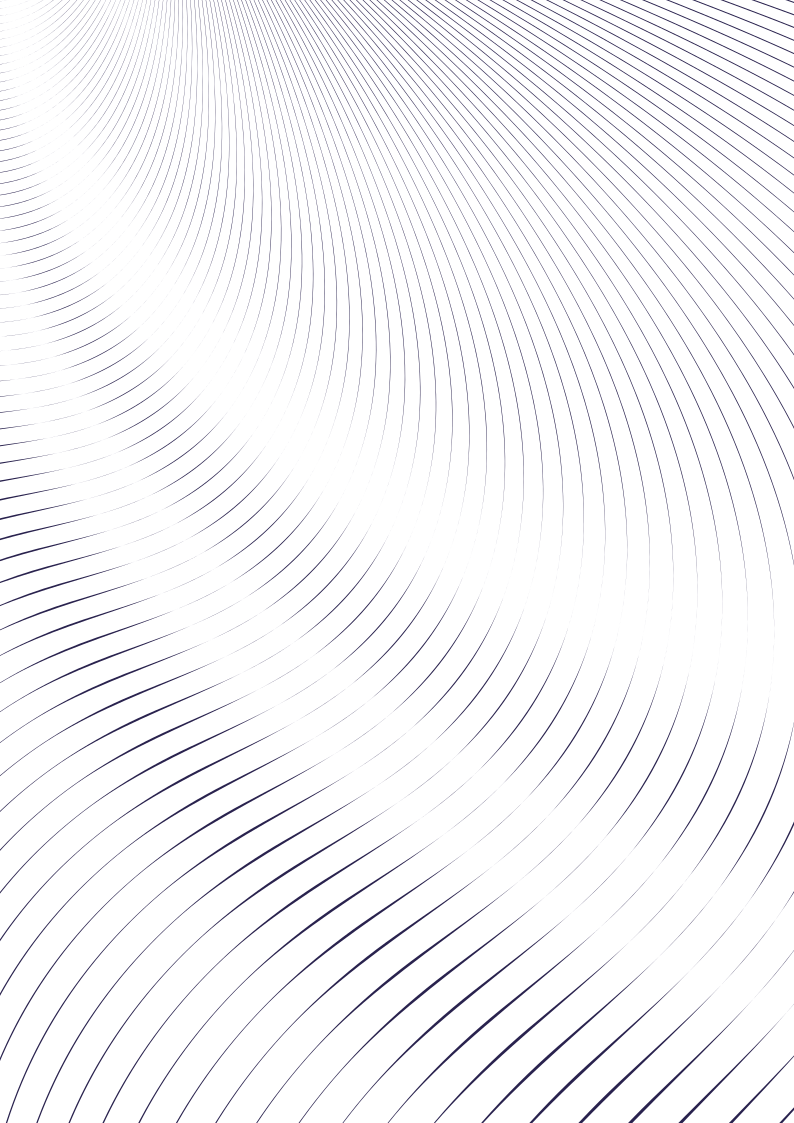
\includegraphics[width=\paperwidth,height=\paperheight]{AAUgraphics/aau_waves}}
    }
		
  \begin{center} %%please do not change the height or width of the frontpage image
    \centerline{\includegraphics[totalheight=0.5\paperwidth,width=1\paperwidth]{AAUgraphics/frontpageImage}}% 
  \end{center}
	
	\vspace*{-0.96cm}
  {\noindent\color{aaublue}\fboxsep0pt\colorbox{white}{\begin{tabular}{@{}p{\paperwidth}@{}}
    \centerline{
    \begin{minipage}{0.85\textwidth}
        \bigskip
				\bigskip
        \centering
        \Huge{\textbf{
A simple explanation of how our Universe was formed% insert your title here
        }}
    \end{minipage}
    }
		
	\centerline{
	\begin{minipage}{0.9\textwidth}
        \bigskip
        \centering
        \Large{
Development of a predictive model% insert your subtitle here
        }
    \end{minipage}
    }
			
	\centerline{
	\begin{minipage}{0.9\textwidth}
        \bigskip
        \centering
        {\Large
Anders Andersen, Alfred Alfredsen, Anne Annesen% insert names separated by comma
        }
    \end{minipage}
    }
			
    \centerline{
    \begin{minipage}{0.9\textwidth}
        \bigskip
        \centering
        {\large
Energy Technology, TEPE4-1005, \the\year-06% insert name of study, group number, year-month
        } 
    \end{minipage}
    }
			
    \centerline{
    \begin{minipage}{0.9\textwidth}
        \bigskip
        \centering
%% Comment this section if you are not doing Bachelor or Master Project   
        {\Large
Master's Project
      %Bachelor Project
        }
        \smallskip
    \end{minipage}
    }
			
  \end{tabular}}}

  \vfill
  \begin{figure}[!b]
	\centering
    
\includegraphics[width=0.2\paperwidth]{AAUgraphics/aau_logo_circle_en}% comment this line in for English version
    %
\includegraphics[width=0.2\paperwidth]{AAUgraphics/aau_logo_circle_da} %comment this line in for Danish version
  \end{figure}
\end{titlepage}
\restoregeometry
\pdfbookmark[0]{Front page}{label:frontpage}%
\begin{titlepage}
\vspace*{\fill}
    \backgroundsetup{
    scale=1.1,
    angle=0,
    opacity=1.0,  %% adjust
    contents={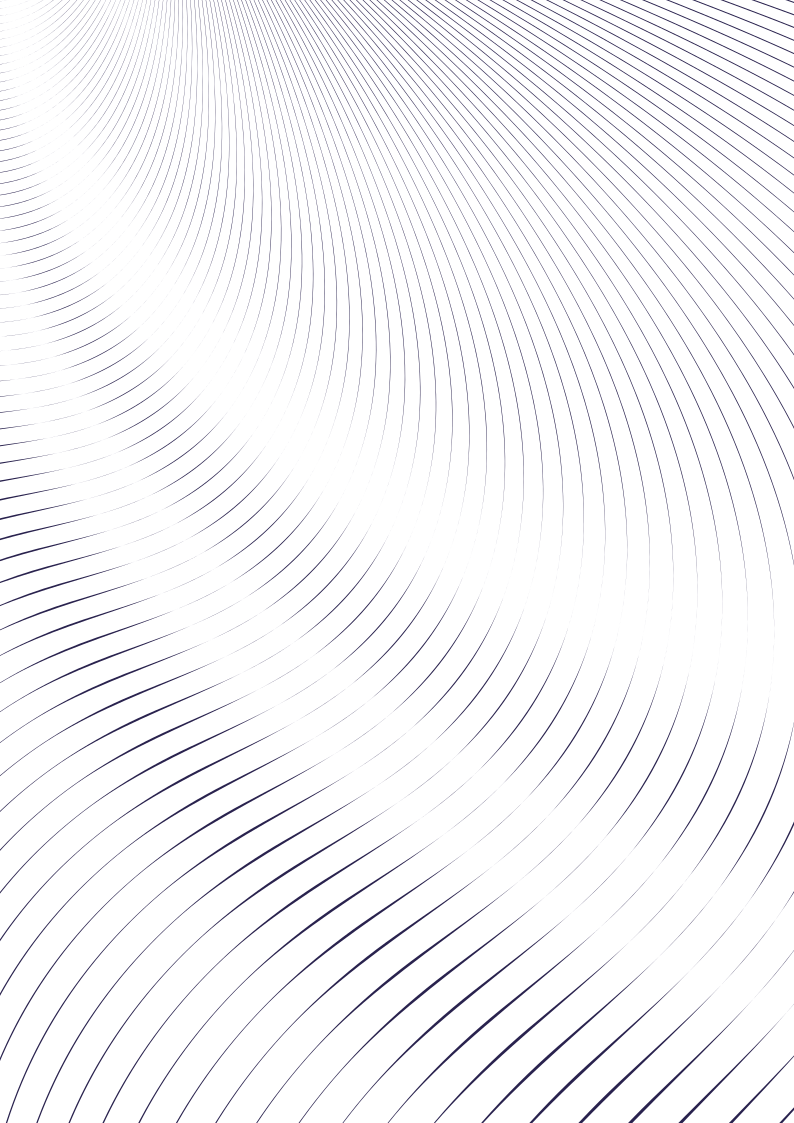
\includegraphics[width=\paperwidth,height=\paperheight]{AAUgraphics/aau_waves}}
    }
  \addtolength{\hoffset}{0.5\evensidemargin-0.5\oddsidemargin} %set equal margins on the frontpage - remove this line if you want default margins
  \noindent%
  {\color{white}\fboxsep0pt\colorbox{aaublue}{\begin{tabular}{@{}p{\textwidth}@{}}
    \begin{center}
    \Huge{\textbf{
      P7 - Teaching Platform
    }}
    \end{center}
    \begin{center}
      \Large{
        Subtitle % insert your subtitle here
      }
    \end{center}
    \vspace{0.2cm}
   \begin{center}
    {\Large
      Christian Bager Bach Houmann, Daniel Overvad Nykjær, Ivik Lau Dalgas Hostrup, Marco Klaustrup Justesen, Patrick Frostholm Østergaard, Rasmus Høyer Hansen % insert names separated by comma
    }\\
    \vspace{0.2cm}
    {\large
      Software Engineering, cs-22-sw-7-09, 2022-12% insert name of study, group number, year-month
    }
   \end{center}
   \vspace{0.2cm}
%% Comment this section in if you are doing Bachelor or Master Project   
   \begin{center}
    {\Large
      7th semester
    }
   \end{center}
  \end{tabular}}}
  \vfill
  \begin{center}
    
\includegraphics[width=0.2\paperwidth]{AAUgraphics/aau_logo_circle_en}% comment this line in for English version
    %
\includegraphics[width=0.2\paperwidth]{AAUgraphics/aau_logo_circle_da} %comment this line in for Danish version
  \end{center}
\end{titlepage}
\clearpage

\thispagestyle{empty}
{\small
\strut\vfill % push the content to the bottom of the page
\noindent Copyright \copyright{} Aalborg University 2022\par
}
\clearpage


\pdfbookmark[0]{English title page}{label:titlepage_en}
\aautitlepage{%
  \englishprojectinfo{
    P7 Programming Paradigms Practice Platform
  }{%
    Internet
  }{%
    Fall Semester 2022 %project period
  }{%
    cs-22-sw-7-09 % project group
  }{%
    %list of group members
    Christian Bager Bach Houmann\\
    Daniel Overvad Nykjær\\
    Ivik Lau Dalgas Hostrup\\
    Marco Klaustrup Justesen\\
    Patrick Frostholm Østergaard\\
    Rasmus Høyer Hansen
  }{%
    %list of supervisors
    Carlos E. Muniz Cuza
  }{%
    N/A % number of printed copies
  }{%
    \today % date of completion
  }%
}{%department and address
  \textbf{Computer Science}\\
  Aalborg University\\
  \href{http://www.aau.dk}{http://www.aau.dk}
}{% the abstract
This report presents a web-based teaching platform with the goal of helping students learn Haskell in a classroom setting. The platform provides a user-friendly interface for creating and solving exercises, as well as a system for managing and organizing the exercises and tracking student progress. By making use of concurrency and queuing mechanisms, the platform can handle many students submitting solutions at once. The platform uses a role-based system for distinguishing user permissions such that lecturers and students can access different parts of the platform. Lecturers are able to create and edit exercises, and view the progress of all students. Students can view their progress and submit solutions to exercises.
}{% keywords
}

% \cleardoublepage
% {\selectlanguage{danish}
% \pdfbookmark[0]{Danish title page}{label:titlepage_da}
% \aautitlepage{%
%   \danishprojectinfo{
%     Rapportens titel %title
%   }{%
%     Semestertema %theme
%   }{%
%     Efterårssemestret 2010 %project period
%   }{%
%     XXX % project group
%   }{%
%     %list of group members
%     Forfatter 1\\
%     Forfatter 2\\
%     Forfatter 3
%   }{%
%     %list of supervisors
%     Vejleder 1\\
%     Vejleder 2
%   }{%
%     1 % number of printed copies
%   }{%
%     \today % date of completion
%   }%
% }{%department and address
%   \textbf{Elektronik og IT}\\
%   Aalborg Universitet\\
%   \href{http://www.aau.dk}{http://www.aau.dk}
% }{% the abstract
%   Her er resuméet
% }}
%
\chapter*{Preface\markboth{Preface}{Preface}}\label{ch:preface}
\addcontentsline{toc}{chapter}{Preface}
Group cs-22-sw-7-09 will hereby be referred to as \textit{our group}, \textit{our}, or \textit{we} for the purpose of this document.
This report is a documentation of the work done by our group in the course of the semester.

We would like to extend our thanks to our supervisor \textit{Carlos} for the support and guidance that we received throughout the semester.

\vspace{\baselineskip}\hfill Aalborg University, \today
\vfill\noindent


\begin{minipage}[b]{0.45\textwidth}
 \centering
 \rule{\textwidth}{0.5pt}\\
 Christian Bager Bach Houmann\\
 {\footnotesize <chouma19@student.aau.dk>}
\end{minipage}

\hfill
\begin{minipage}[b]{0.45\textwidth}
 \centering
 \rule{\textwidth}{0.5pt}\\
  Daniel Overvad Nykjær\\
 {\footnotesize <dnykja18@student.aau.dk>}
\end{minipage}

\begin{minipage}[b]{0.45\textwidth}
 \centering
 \rule{\textwidth}{0.5pt}
  Ivik Lau Dalgas Hostrup\\
 {\footnotesize <ihostr16@student.aau.dk>}
\end{minipage}

\hfill
\begin{minipage}[b]{0.45\textwidth}
 \centering
 \rule{\textwidth}{0.5pt}
  Marco Klaustrup Justesen\\
 {\footnotesize <mkju19@student.aau.dk>}
\end{minipage}

\begin{minipage}[b]{0.45\textwidth}
 \centering
 \rule{\textwidth}{0.5pt}
  Patrick Frostholm Østergaard\\
 {\footnotesize <pfas19@student.aau.dk>}
\end{minipage}

\hfill
\begin{minipage}[b]{0.45\textwidth}
 \centering
 \rule{\textwidth}{0.5pt}
  Rasmus Høyer Hansen\\
 {\footnotesize <rhha19@student.aau.dk>}
\end{minipage}
\cleardoublepage
\pdfbookmark[0]{Contents}{label:contents}
\pagestyle{fancy} %enable headers and footers again
\tableofcontents
%\listoftodos
\cleardoublepage
%mainmatter
\pagenumbering{arabic} %use arabic page numbering in the mainmatter

% ! Place your sections here !

\chapter{Introduction} \label{chap:introduction}
\chapter{Introduction} \label{chap:introduction}
On the 1st semester of the Software Master’s Degree at \aau{}, the Programming Paradigms course had a problem where most attending students failed the course last year. 
This resulted in a survey being sent out, and a student task force being assembled to grasp the main flaws with how the course was structured. 
Here, many students mentioned lacking experience in the programming languages taught in the course given few opportunities to actively train their skills during the semester. 


With this in mind, \aau{} chose to restructure the course entirely. 
The course now focuses on a single programming language instead of multiple. 
Furthermore, the course features more practical programming instead of following the traditional lecture model usually used at universities. 
To support this way of teaching, the course lectures have been moved to a more classical classroom setup, but with a monitor at each table and a main monitor at the lecture desk. 
This is meant to allow students to more easily work together in groups by using the shared monitor.
In addition, it allows the professor to view and share other groups' monitors such that student solutions can used for classroom discussions. 


This new approach causes its own problems, however. 
Since students use their own local development environments for solving exercises, other students cannot revisit the discussed exercise solutions as these are not shared, making it impossible to revisit them later. 
Furthermore, it is difficult to verify whether your own solution is correct and lives up to the requirements of the exercise. 
In fact, it is not uncommon for people to accidentally misunderstand an exercise and therefore implement an incorrect solution.

\section{Initial Problem} \label{sec:initial-problem}
The restructuring of the course already seems like a major improvement over the former structure, but as mentioned it still suffers from a few notable problems related to the execution of the exercise sessions:
\begin{itemize}
	\item No way to revisit discussed solutions
	\item No way to verify that your own solution is correct
	\item No way for the entire group to work together on the same code
	\item No way for the professor to verify how many exercises the students have solved
	\begin{itemize}
		\item Difficult to verify that all students have solved the problems
		\item Difficult to judge the skill level of the students and whether the difficulty of exercises is suitable
	\end{itemize}
\end{itemize}

By summarizing the main problems following the switch to a more practical and exercise focused teaching environment, an initial problem statement can be written.
\begin{displayquote}
How can one ensure a mutual feedback loop between students, TAs and the professor during exercise session?
\end{displayquote} 

\subsection{Minimal Viable Product}
Considering that students use a variety of different operating systems, a web application would be the best way to ensure easy portability.
To facilitate the problems mentioned in \ref{sec:initial-problem}, we imagine a website that allows users to complete the following tasks:
\begin{itemize}
	\item The professor should be able to create a syllabus with exercises that students are expected to solve
	\begin{itemize}
		\item The professor should be able to create multiple syllabi where students can self-enroll
	\end{itemize}
	\item The professor should be able to track the amount of exercises solved by each enrolled student
	\begin{itemize}
		\item The professor should be able to view additional statistics like the number of attempts used by a student to solve an exercise
	\end{itemize}
	\item The professor should be able to specify criteria in order to pass each exercise 
	\begin{itemize}
		\item Students should be able to verify whether their solution is correct
		\item Verifying solutions should be automatically handled by the system
	\end{itemize}
	\item Students should be able to collaborate on the same code
	\item Students should have access to discussed solutions later on
	\item The professor should be able to see each students code
\end{itemize}

The presented features were then prioritized by a group of students to construct a minimal viable product (MVP) that could be tested and used to verify if the presented product would provide anything useful to the course. Since the MVP is meant to be used as a demo product that allows for additional input to be gathered only the minimum number of functionalities needed were included.

\begin{displayquote}
A website that allows a user to specify a set of exercises as well as the completion criteria for each of these exercises. Furthermore an option to verify whether the submitted code is a correct solution to the chosen exercise.
\end{displayquote}






\chapter{Preliminaries} \label{chap:preliminaries}
\input{sections/Chapter 02 - Preliminaries/Preliminaries}
\chapter{Specification} \label{chap:Specification}
This chapter presents an overview of our system using a system specification containing the purpose and the scope of our system, the target users, the constraints of the project, the use cases, and the prioritization using a MoSCoW analysis.

\section*{Purpose and scope of the system }
The purpose of the system is to provide a better approach to learning functional programming in Haskell using a software application.
We aim to make a system where students can solve exercises. The system should be able to provide feedback on whether the user's solution compiles, and whether it fulfills the requirements of the exercise. 
In addition, the lecturer should be able to add exercises and write specifications for exercise solutions.

To reduce the scope of the project, we choose to focus on creating a platform for the \textit{Programming Paradigms} course, while ensuring the system abstractions support other languages, that could be supported in the future.
Currently \todo{find number} students attend the course, thus we do not expect many of the following usecases to be performed at the same time. 
We will use the number of course attendees to create an estimation of an operational profile which will be used to stress test the solution, as described in \ref{chap:Benchmarking}

\section*{Target users}
The system will have two main users, the lecturer that will conduct the course, and the university students who will take the course.
Therefore the responsibility of the frontend can be split into two categories: 
\begin{itemize}
    \item \textbf{Lecturer}-based responsibilities.
    \item \textbf{Student}-based responsibilities.
\end{itemize}

\subsubsection*{Lecturer-based responsibilities}
If the signed in user is a lecturer the frontend provides the lecturer the ability to create syllabi, sessions, exercises and test cases for the exercises, as well as they ability to solve and submit exercises. The ability for the lecturer to solve and submit exercises was included to allow lecturers to try out the exercises and ensure that the test cases behave as expected before releasing the exercises to the students. Additionally, the lecturer will also have access to a dashboard that shows which students have completed which exercises for a given session, in order to track progress and .

\subsubsection*{Student-based responsibilities}
Conversely to the Lecturer-based responsibilities, if the signed in user is a student, the fronted provides the user the ability to view syllabi, sessions and exercises as well as the ability to attempt exercises. A student will also have access to an overview showing which courses are available to the student and which exercises have been completed. 


\section*{Constraints of the project}
Given this project is developed as a semester project at \aau{} there will be some constraints that we must adhere to. 
One of the constraints is the time constraint: we have a single semester, or approximately 3 months, to develop the system. 
In addition, we should design an internet based system that is scalable. 
 
\section*{Use Cases} \label{sec:use_cases}
The goal of the project is to improve the teaching methods applied to the \textit{Programming Paradigms} course. 
To best assess whether the project solves the current issues related to the course, and therefore improves it, we will describe use cases in an application which satisfies this goal.
Use cases also allows us to prioritize the features needed later on.
The following sections contain the use cases we have outlined that fall under our scope in no particular order.  

\subsection*{Use case: Accounts}
To keep track of what exercises each user has solved, and which permissions they have, a user should be able to log in to the platform, and be registered as a student or a lecturer.

\subsection*{Use case: Solve exercises}
A Student should be able to choose an exercise session and a specific exercise. The exercise description is then retrieved and shown to the user.
As the user completes the exercise, they should also be able to submit the exercise, and verify that their submitted solutions can compile and fulfills the requirements of the exercise. If it does not compile or fails the tests, it should provide the user with an error describing the problem. 

\subsection*{Use case: Create exercises}
A Lecturer should be able to create and edit syllabi as well as the belonging exercise sessions and their included exercises. 
For each given exercise the user should be able to specify an exercise description and tests that must be passed, the tests should be performed on the submitted code. Furthermore the Lecturer should be able to specify template code that will already be entered when the students opens the exercise.

\subsection*{Use case: Show statistics over exercises}
A Lecturer should be able to view statistics about exercises, for example how many attempts were needed by the Students to complete it or the time taken, in order to determine if the difficulty is sufficient. To do this the system needs to log the information as the users attempt to complete the exercises.

\subsection*{Use case: View solutions}
The Lecturer can view all submitted solutions, to see if the students use the correct approach.
The Students should be able to view their own solutions and attempts for the exercises.
To do this a database keeping a track of the code used for each attempt submitted is needed. 

\subsection*{Use case: Best solutions} 
The Lecturer should be able to select code solutions submitted by the Students to publish to all other Students allowing them to view exercises discussed during class.

With the use cases that are contained in our scope described, we need a way to prioritize them. This then allows us to make a prioritized list of the features that are needed in-order to fulfill our use cases. 

\section{MoSCoW}
To gain an overview of which features the solution must, should, could and won't contain we perform a MoSCoW analysis.
A MoSCoW analysis is split into four categories, Must have, Should have, Could have and Would have. Each feature will then be put into a category based on how important it is for the system. 

Table \ref{tab:MOSCOW} shows the feature prioritizations for a working solution. 

The must have section includes the features required for students to solve exercises. These are seen as must-have features as all use cases other than the Account one require these.  
The should-have category includes the additional features that are needed to fulfill the Solve Exercises use case as well as the Create Exercise one. 
These are prioritized as should have as they are needed in order to provide the users with the main expected features of an exercise platform for coding. 
Account Handling, as well as exercise attempt logging features, are placed in the could have category as they are both nice to have but indeed needed in order to provide a usable solution. 
Lastly, statistics and solution highlighting are placed in the wont have category as they have been deemed out of scope according to the constraints of the problem.


% Please add the following required packages to your document preamble:
% \usepackage[table,xcdraw]{xcolor}
% If you use beamer only pass "xcolor=table" option, i.e. \documentclass[xcolor=table]{beamer}
\begin{table}[H]
    \begin{tabular}{|l|llll}
    \cline{1-1}
    \cellcolor[HTML]{C0C0C0}\textbf{Must have}                                    &  &  &  &  \\ \cline{1-1}
    Students can retrieve exercise descriptions                                   &  &  &  &  \\ \cline{1-1}
    Students can submit exercise attempts                                         &  &  &  &  \\ \cline{1-1}
    The system can interpret exercise attempts                                    &  &  &  &  \\ \cline{1-1}
    Lecturers can group exercises into sessions                                   &  &  &  &  \\ \cline{1-1}
    \cellcolor[HTML]{C0C0C0}\textbf{Should have}                                  &  &  &  &  \\ \cline{1-1}
    Lecturer can add tests for exercises                                          &  &  &  &  \\ \cline{1-1}
    The system can verify if the students exercise attempt completes the test     &  &  &  &  \\ \cline{1-1}
    Users can login to determine if they are a student or a lecturer              &  &  &  &  \\ \cline{1-1}
    \cellcolor[HTML]{C0C0C0}\textbf{Could have}                                   &  &  &  &  \\ \cline{1-1}
    Students can access old exercise attempts                                     &  &  &  &  \\ \cline{1-1}
    Lecturer can view all exercise attempts submitted by students                 &  &  &  &  \\ \cline{1-1}
    \cellcolor[HTML]{C0C0C0}\textbf{Wont have}                                    &  &  &  &  \\ \cline{1-1}
    Lecturer can share submitted solutions so they are viewable by other students &  &  &  &  \\ \cline{1-1}
    Lecturer can access statistics over the exercise attempts                     &  &  &  &  \\ \cline{1-1}
    \end{tabular}
    \caption{\label{tab:MOSCOW}MoSCoW Analysis}
\end{table}

The \textit{Must have} category from the MoSCoW analysis represents the minimal amount of features that we want to include to satisfy the goals of the project. Throughout the report we will refer to this as the Minimal Viable Product (MVP).
In the following chapter we will describe the design of the system which is based on the MVP. 
    


\chapter{Design} \label{chap:Design}
\chapter{Architecture} \label{chap:Architecture}
\chapter{Test Runner} \label{chap:TestRunner}
One of the primary goals of this application to give the professor a way to specify what constitutes a correct problem solution.
As previously mentioned in the \textbf{Use Cases} section of chapter \ref{chap:Specification}, a common approach to this is the use of test cases.

\section{Client-Server Interaction}
When a teacher creates a new exercise, a modal prompts them to enter details about the exercise.
These details include the name of the exercise, instructions for the student, an optional code template to help the student get started, as well as test code.
This data is sent to the database where it is stored.
When a student opens an exercise, the data is then fetched from the database.
This is done by the client sending a request to the Next.js backend, which queries the database and returns both exercise and test data.

\begin{figure}[H]
    \centering
    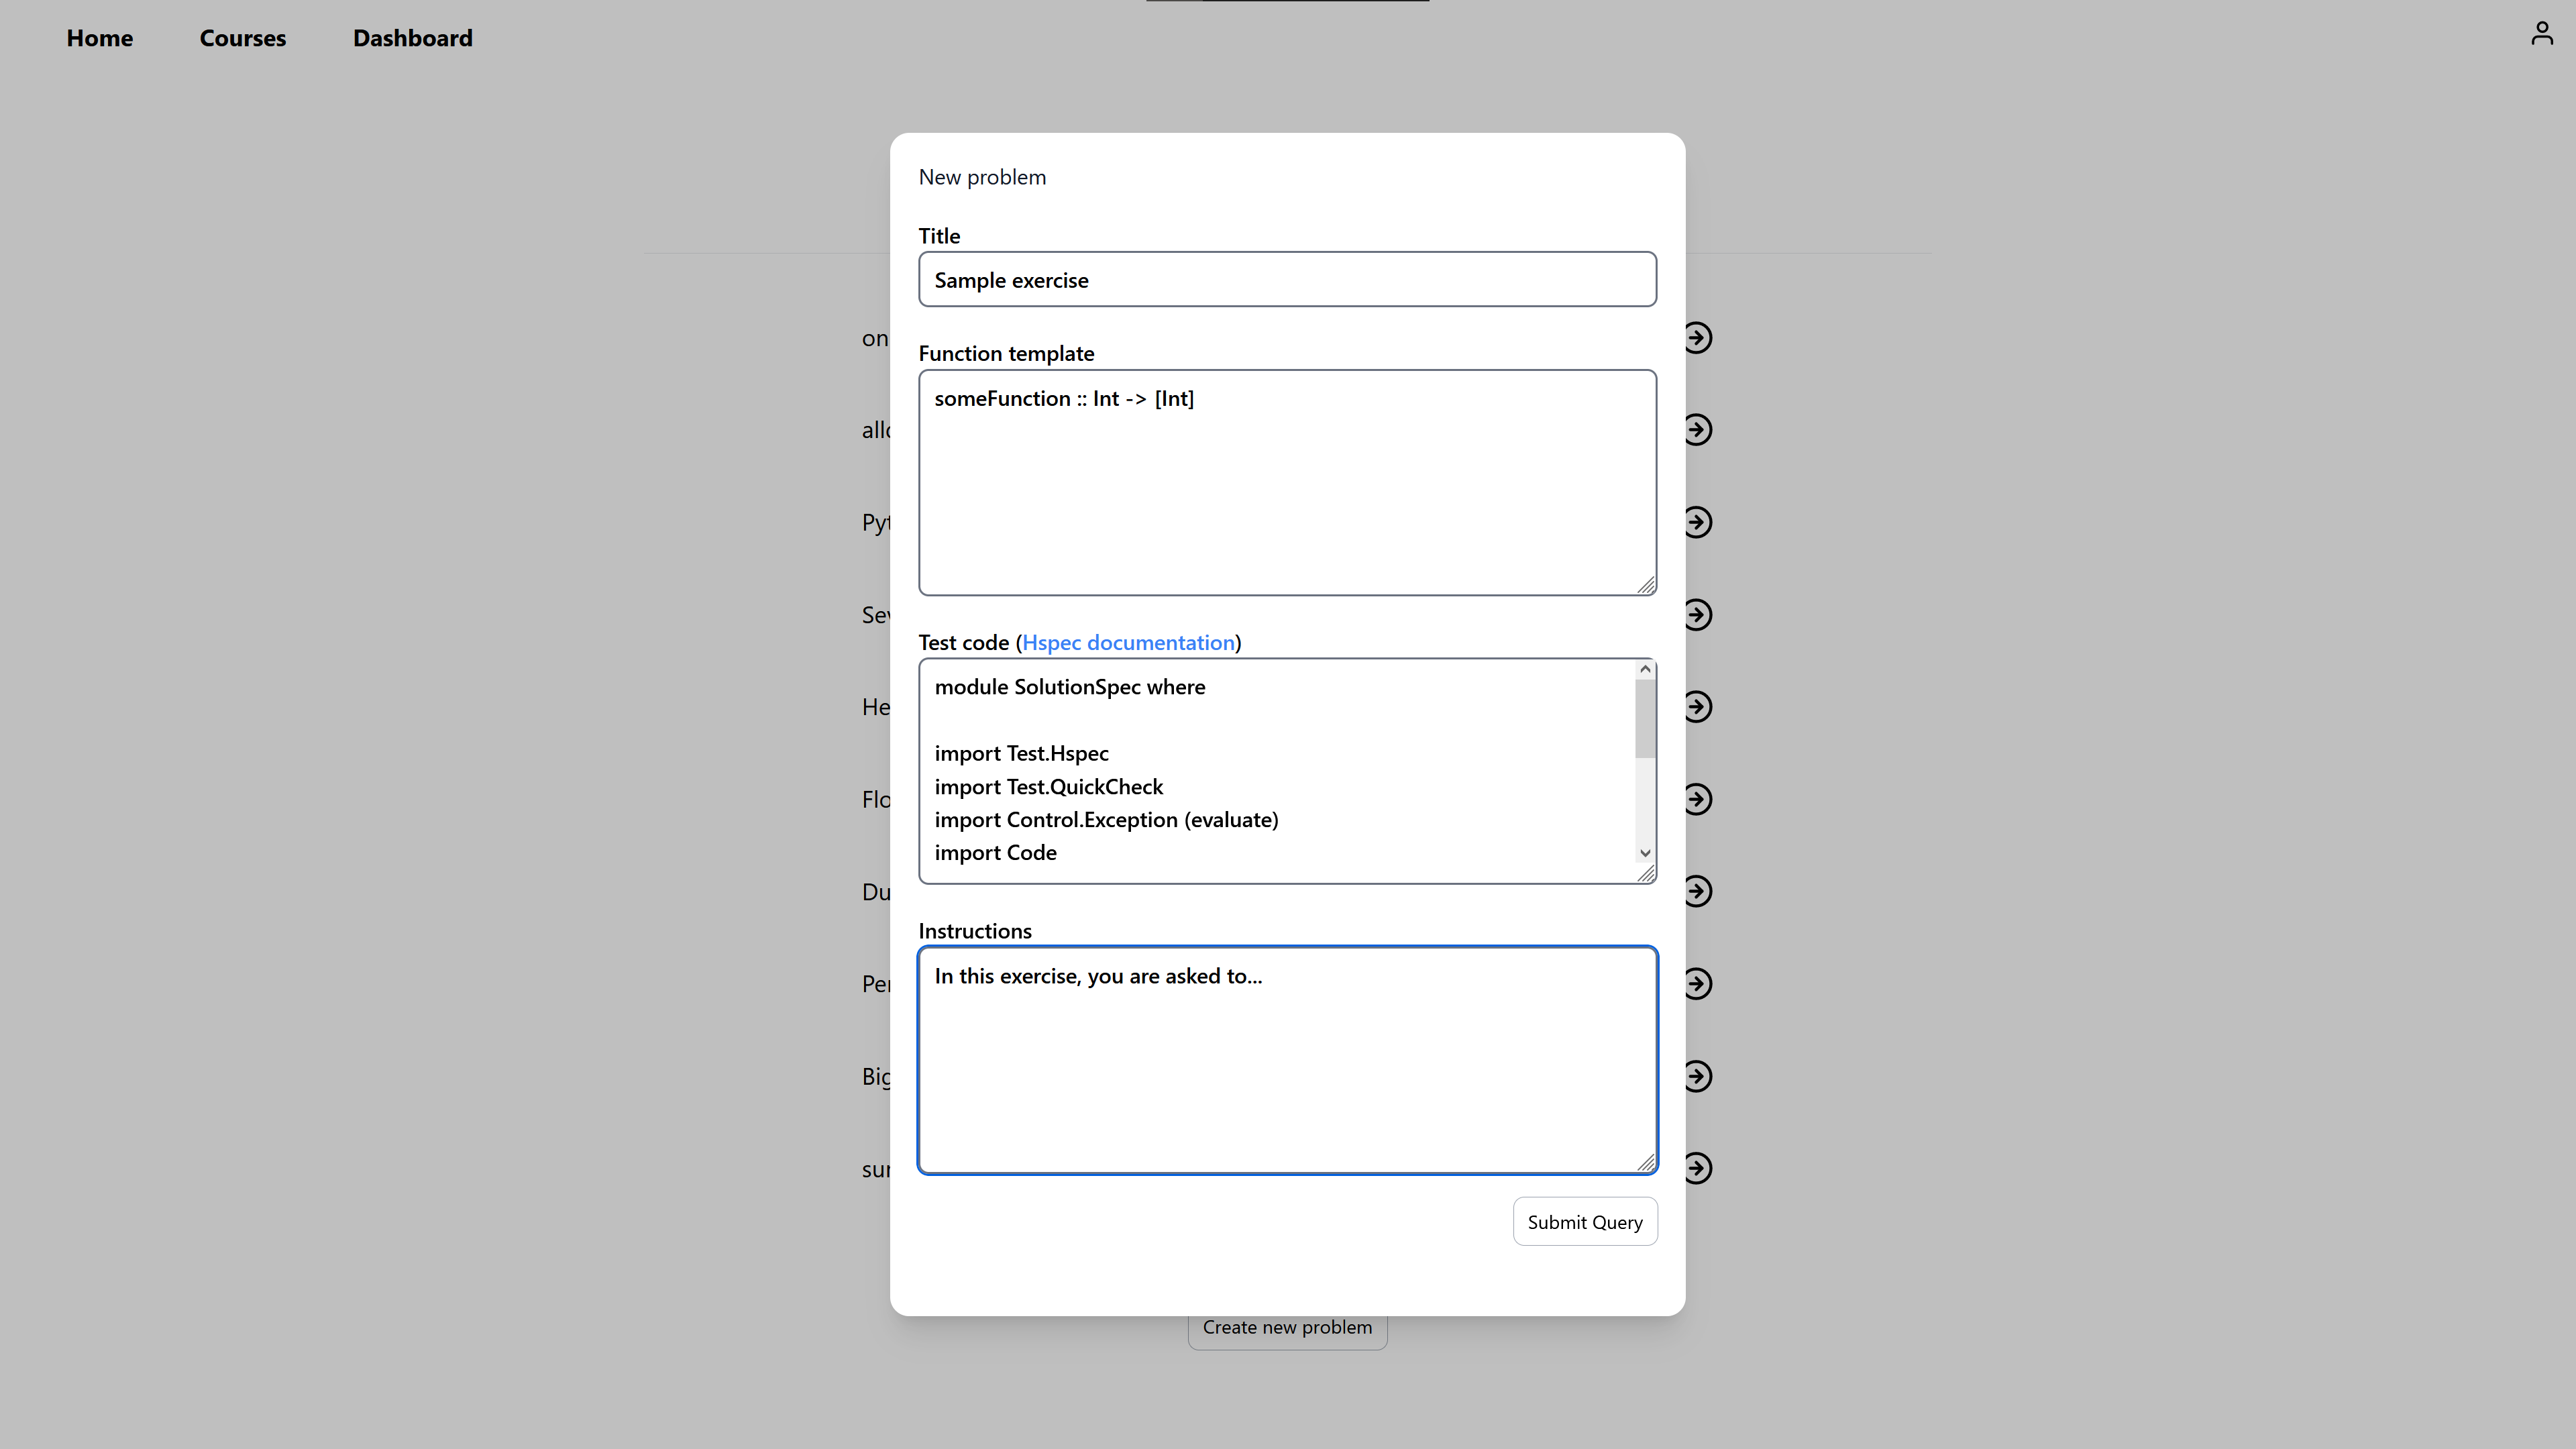
\includegraphics[scale=0.1]{create_exercise.png}
    \caption{Creating a new exercise as a teacher.}
    \label{fig:create_exercise}
\end{figure}

In the interest of reducing the number of database queries, the result of this request is cached on the client.
The client will eagerly request new data to stay up to date with instructions or test code updates.
We deemed that this short cache storage time is useful for when teachers update test code during an exercise session.
This way, all students have the latest test code shortly after the update while still minimizing unnecessary queries.

When a user submits their exercise solution attempt, a mutation is sent to the Next.js backend.
In this request, the necessary code and test code is included.
One could argue that fetching the test code on the backend when processing this mutation would be more appropriate.
However, we want to eventually display the test code to the user so they may gain a better understanding of the solution requirements, although this will not be done in this iteration of the project.

To handle this mutation, the Next.js server requests the Test Runner to process the given solution and test code.
This process is described in section \label{sec:test_runner_process} below.
The response of this request to the Test Runner is validated and stored as a submission in the database.
This allows users and teachers to access previous submissions, which includes code and a value indicating whether the submission satisfied the exercise tests.

Lastly, the result is sent to the client and displayed on the page.

\begin{figure}[H]
	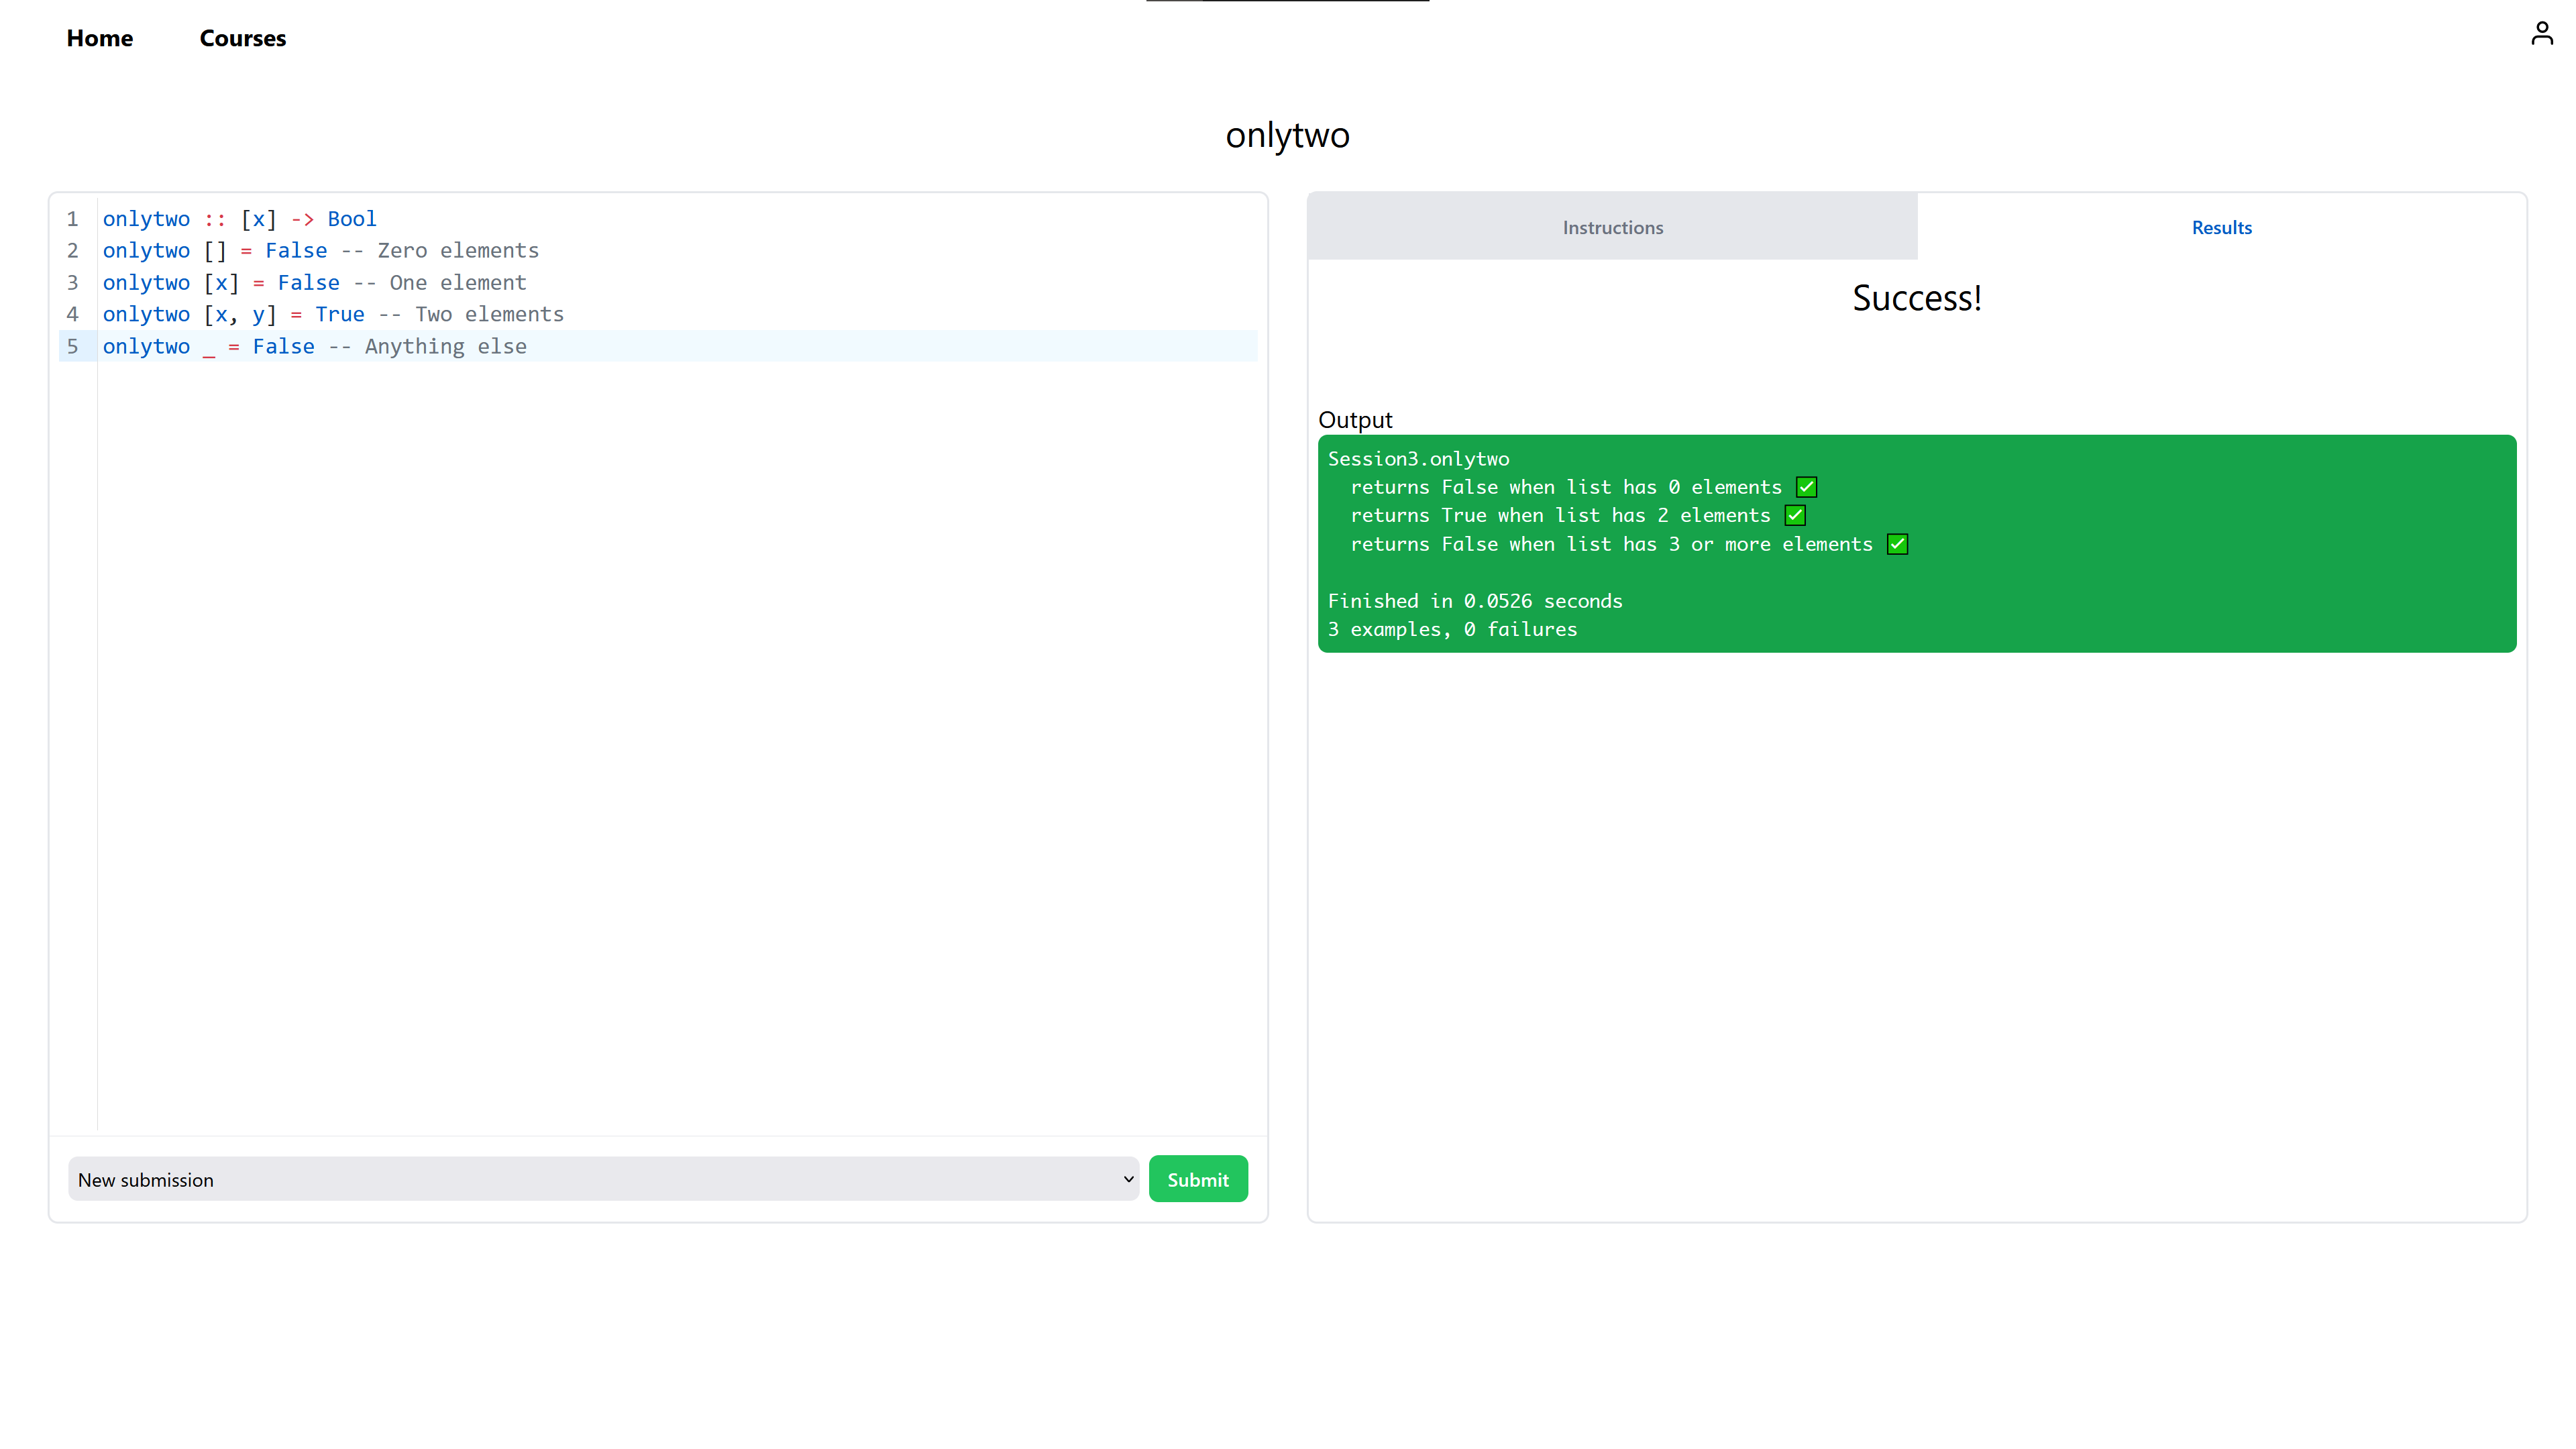
\includegraphics[scale=0.1]{exercise_success.png}
	\centering
	\caption{An example of a successful exercise submission.}
	\label{fig:exercise_success}
\end{figure}

\begin{figure}[H]
	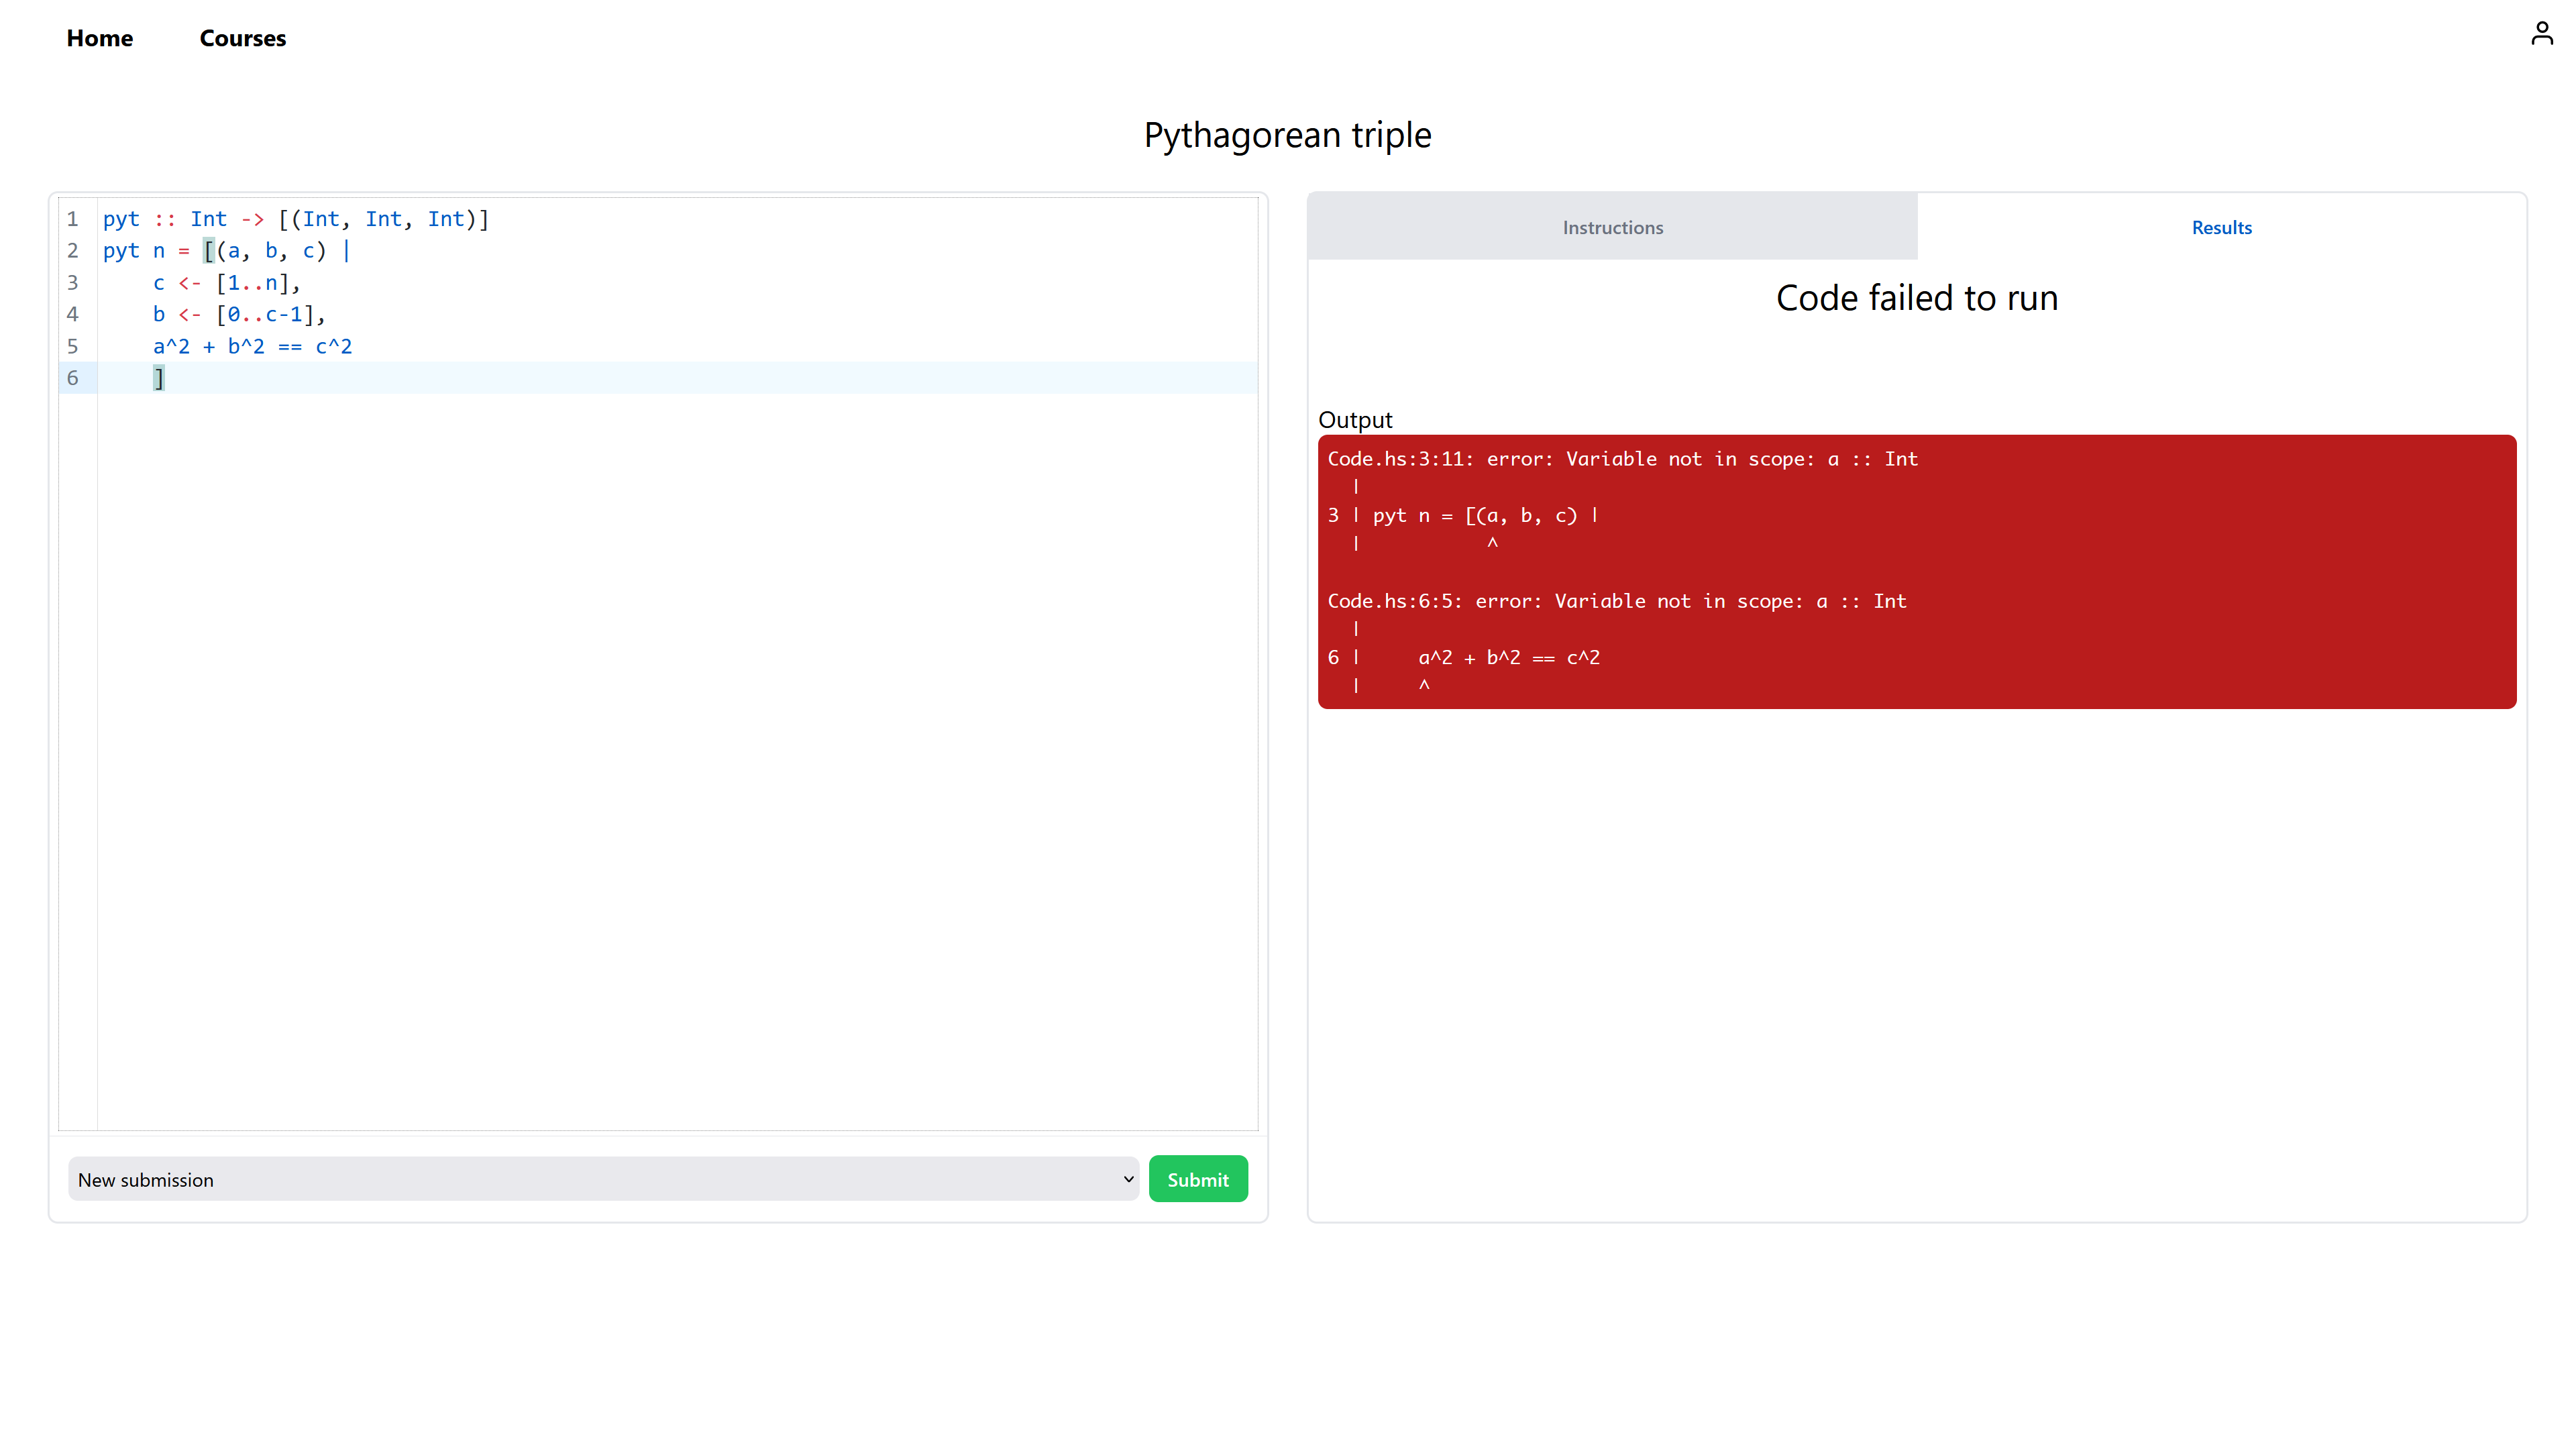
\includegraphics[scale=0.1]{exercise_fail.png}
	\centering
	\caption{An example of an unsuccessful exercise submission.}
	\label{fig:exercise_fail}
\end{figure}

More images of the platform user interface can be seen in chapter \ref{chap:images} in the appendix.


\section{Test Runner process} \label{sec:test_runner_process}
The Test Runner exposes an endpoint \texttt{/haskell/submit/}, which is used to post code submissions.
Originally, we used the Rust crate Rocket to implement this endpoint.
However, we eventually switched to using the axum crate instead, as it is developed and maintained by the same developers behind the Tokio package we make heavy use of for asynchronous programming and multithreading.
Furthermore, it was deemed easier to implement a shared state among endpoints by leveraging axum's \texttt{layer} feature.
We give an overview and a more technical explanation of how this was done in section \ref{sec:queue-system}.

When the Test Runner receives the request from Next.js, its singular goal is to run the tests against the code and send the result of this back as fast as possible.
In order to run the tests, we need to run the GHC interpeter on the test code, which, in turns, need access to the exercise submission code.
The GHC interpreter can be run from the command line with arguments specifying the path Haskell file to run.
In other words, the Test Runner needs to write the user submission and corresponding test code to a file.
However, if more users were to make a submission at the same time, the content of the file could potentially be overwritten while the GHC interpreter is running the tests.

To address this, we generate a new directory with a unique name for each submission.
Then, the user submission is written to two  \texttt{.hs} files inside this directory - a \texttt{code.hs} file containing the exercise submission, and a \texttt{test.hs} file containing the corresponding tests.
This way, we can pass the path to this isolated directory to the GHC interpreter process as an argument.
Once the tests have been run, the directory and its contents are deleted again.
The \texttt{stdout} of the process is then read to determine whether the tests succeeded or not.
Finally, the interpreter output and the test success flag is packaged into a JSON object and sent back to the client.

Sequentially starting a new \texttt{runhaskell} process for each request was identified as a major bottleneck during testing, which will be described in detail in chapter \ref{chap:Benchmarks}.
In order to address this, we started by refactoring the code base to allow running several instances of the GHC interpreter process at the same time.
However, despite this running faster for a small number of clients, this approach in itself is not sufficiently stable:
If multiple clients were to post a code submission at the same time, the Test Runner will start a new process for each request.
Given a large enough number of requests, this would crash the Test Runner web server.
Therefore, we needed a way to limit the number of running GHC interpreter processes while at the same time storing subsequent requests for future processing.
 \chapter{Queue System} \label{chap:QueueSystem}
In chapter \ref{chap:TestRunner}, we described how running multiple GHC interpreter processes asynchronously eventually crashes the test runner web server given sufficiently many simultaneous requests.
As mentioned, we needed a way to limit the number of running GHC interpreter processes in order to prevent crashes.
In the following sections, we first give a general overview of how this was implemented.
We then describe the technical approach in more detail.

\section{Overview}
To solve the aforementioned problem, we decided to implement a queue system which enqueues requests for future processing if some upper limit is reached.
However, this introduces a new problem.
The server can no longer directly respond to a POST request with the test runner results because the request may be handled at a later point in time.
This means that if the request were enqueued for long enough, it would eventually time out.
In order to solve this, the test runner web server sends back a unique token to the client immediately upon receiving a POST request.
This token serves as a ticket for the client. 
Using it, the client can continuously poll the server for the result of processing the request.
To achieve this, we implemented a new endpoint which expects the token as a parameter.
There are three possible responses from this endpoint:
\begin{enumerate}
    \item If the given token is not present within the queue, the response body contains a special "not found" message.
    \item If the given token is present within the queue but has not yet been processed, the response body contains a special "in progress" message.
    \item If the given token is present within the queue and has been processed, the response body contains a special "complete" message as well as the results of running the tests on the submitted code from the request.
\end{enumerate}

In summary, the test runner web server features two endpoints.
The first endpoint expects a POST request containing a code submission which it enqueues into a worker queue along.
It then responds to the client with a unique token.
This token is also used by the web server as a key to look up the given code submissions in the queue.
The second endpoint expects a GET request with a token as a parameter that is then used to look up the result of processing the code submission with the matching token ID.
It then responds to the client with the result of processing that submission if it was found.

\section{The queue}
We have two endpoints that need to share data, and the Rust programming language does not allow global variables.
Therefore, we opted to create a shared state data structure using the \texttt{layer} feature in the axum framework.
The \texttt{layer} feature is axum's default implementation of middleware for processing data across a group of endpoints.
In our case, there are two key variables inside the shared state structure that both endpoints need access to:
\begin{enumerate}
    \item \textbf{A sender channel:} In practice, this channel is used as a worker queue in which code submission requests are enqueued for processing. It has a corresponding \textbf{receiver channel}, which is to dequeue and schedule work. Importantly, requests sent via the sender channel are received in a first-in-first-out order.
    \item \textbf{The job results hashmap:} Upon first receiving a code submission request, a unique token is generated and used as a key to reference an empty piece of work inside the hashmap. When the test runner has processed the code submission, it inserts the result of the work in the hashmap as the value in the hashmap using the token as the key. This value can then be looked up when the client requests the result processing their code submission, since the client is provided with the token upon sending a code submission, as previously mentioned.
\end{enumerate}

In order to limit the number of GHC interpreter processes, a thread pool with a specified size is created whose responsibility is to process code submissions.
These threads have access to the aforementioned receiver channel containing work to be processed.
The creation and content of the the thread pools can be seen in code snippet \ref{lst:worker-thread}.

\begin{lstlisting}[language=rust, escapechar=|, caption={Rust code showing allocation of thread pools and scheduling of code submission processing.}, label={lst:worker-thread}]
async fn worker_thread(
    rx: Receiver<TestRunnerWork>,
    job_results: Arc<Mutex<Box<HashMap<Uuid, Option<TestRunnerResult>>>>>,
    limit : usize
) {
    let stream = tokio_stream::wrappers::ReceiverStream::new(rx);
    
    stream.for_each_concurrent(limit, |work| async {
        debug!("Running worker thread on UUID {}...", work.id); |\label{line:concurrent-start}|

        let res = schedule_test(work.submission).await;
        let mut map = job_results.lock().unwrap();
        map.insert(work.id, Some(res)); |\label{line:concurrent-end}|
    }).await;
}
\end{lstlisting}

We use the \texttt{futures} package in Rust to allocate some number of threads dictated by the variable \texttt{limit} of type \texttt{usize}.
The receiver channel is converted to a \texttt{ReceiverStream} using the \texttt{tokio\_stream} utility pacckage.
A \texttt{ReceiverStream} is simply a wrapper which implements the \texttt{Stream} trait from the \texttt{futures} package.
This allows us to combine functionality from the two packages.
In practice, implementations of the \texttt{Stream} trait simply provide a stream of values asynchronously --- essentially an asynchronous iterable.
Using this, we can call \texttt{for\_each\_concurrent} from the \texttt{futures} package to run a number of tasks asynchronously but with the aforementioned limit. 
The \texttt{futures} framework then manages the thread pool automatically, and we only need to specifiy the work that the threads need to do, which can be seen in lines \ref{line:concurrent-start} --- \ref{line:concurrent-end}.
 \chapter{Sweeping} \label{chap:Sweeping}
\chapter{Evaluation} \label{chap:Evaluation}
\section{UI evaluation}
To evaluate the User interface of our system, a usability test was conducted using participants that matches our target users. From this test we wanted to determine if our system provides a good user experience, and whether the users feel it is an improvement of the current system.
To do this we use the SUS questions as a basis for our questionnaire, with some added questions in the same format as SUS. The added questions are:
\begin{itemize}
    \item I found the error descriptions clear enough.
    \item I found the overall system could be an improvement to the course.
\end{itemize}
The participants of the usability test are students on the first semester of their Software masters degree who are currently taking the Programming Paradigms course. 
These students have a good understanding of how to use haskell to solve simple exercises, based on this we expect them to be able to successfully use our system. They also have experience with how the course is currently run, and can therefore give feedback on whether it is an improvement.

The usability test will be conducted in a group room with other students present but not interacting with the participant, this will simulate a class setting. 
The equipment used will be the participants own laptop, which simulates use in a real world setting.

\subsection*{Tasks}
To conduct the usability test, we have created a series of tasks that the participants should complete, in order to experience all features of the system.

\begin{enumerate}
    \item In this semester, find exercise "only two" in the "functions and lists" problem set.
    \item Submit a program that should not solve the exercise.
    \item Submit a program that solves the exercise.
    \item Go back to the dashboard.
    \item Check which exercises has been completed by you.
\end{enumerate}

% teachers perspective
    % 1.	tjek hvilke elever der har løst opgave 2
    % 2.	åben daniels løsning
    % 3.	opret et nyt kursus
    % 4.	opret en ny kursusgang
    % 5.	opret en ny opgave


\subsection*{results}

\chapter{Discussion} \label{chap:Discussion}
% State of system -> Discussion -> Future Works
% Bring up what has and hans't been completed from the MoSCoW analysis
\chapter{Reflection} \label{chap:Reflection}
In the following section we will describe how the project was managed, which techniques were used, as well as which issues we encountered. Throughout we will reflect on the decisions that were made in this context.

\section{Task Management}
One of the primary objectives in any project is to manage the tasks that are generated throughout the project. The goal is to maintain an overview of what has been done, what needs to be done and how the tasks are distributed between developers. Additionally, project managers also often want to be able to estimate how long tasks may take to complete and their difficulty. To accomplish this, projects may utilize several project management tools and techniques. In this section we will focus on the tools that we utilized, while in section \ref{sec:agile-dev} we will focus on the techniques that were utilized to manage the project.

\subsection{Github Projects}
GitHub Projects seemed promising, as it integrates with existing developer workflows. You track issues, and as you work on them, they flow from the backlog to \textit{in progress}, to \textit{in review}, and then is at last categorized as \textit{completed}. When you submit a pull request, it goes to the review section, so other members are aware that it is pending. And when that pull request is merged, it goes to completed automatically.
Intuitively, it makes sense to track issues like this, as it is so closely aligned with the modern Git workflow on GitHub. To start contributing to a codebase, you create a branch. Then you reference issues when you make a pull request, which will then become linked to your changes, making issues closely tied to actual code changes.
However, we found that some members were not accustomed to this way of working, and as such, did not take the extra steps to facilitate the automation, such as marking issues as related to the project.
When you create a pull request without referencing issues related to the project, you have to manually assign things later. Given that a pull request does not always correlate directly with issues, this is easily forgotten.
Managing a project generally includes managing non-technical tasks as well, which is hard to track with Projects, as it is very development-specific.
What finally led us to consider other tools were bugs related to the automated workflows not being invoked, resulting in confusion.

\subsection{Notion}
Notion is a platform that allows users to organize resources and manage projects in the same space. The platform allows you to customize the layout of your work space in a way that best suits the team. One particular feature of Notion that we used in this project was the Kanban board. In the Kanban board we defined four categories, similar to what we had in Github Projects, in which we could place work items:

\begin{itemize}
    \item Not started
    \item In progress
    \item Review required
    \item Done
\end{itemize}

While Notion provides fewer features in terms of integration with Github, the tool was familiar to us and provided the functionality that we needed to manage the project.
Once we switched to Notion, planning and updating the tasks became a more active part of our daily work. This led to better productivity as we were now able to better maintain an overview of what each member of the group was doing and and how far they were with each task.

\section{Agile Development Approach} \label{sec:agile-dev}
Irrespective of which tools we used, the goal from the beginning of the project was to use a Scrum-like approach to project management.
The decision to this approach was based on previous experience working with a more rigid Scrum methodology in a school project setting which we had found to be less productive.
Generally, Scrum is a framework that helps teams and organizations generate value through flexible solutions to complex problems. Scrum is an iterative and incremental approach to project work where the project is broken up into sprints. A sprint being a time frame, usually 1-4 weeks in length, in which the the teams tries to complete the work that has been selected from a product backlog\cite{sutherlandScrumArtDoing2014}.

We only adopted the specific things from Scrum that we felt were necessary. For our project we did not have a Scrum master or product owner. Instead, we collectively created tasks based on features that we felt were necessary to implement.
In traditional Scrum, you would have product owners that talk to customers about which features are important to them. Since all group members are both stakeholders and developers, we found that acting as a council is more effective than delegating the role to a single member.

Additionally, instead of traditional sprints, we designed the specifications for a minimum viable product, consisting of only the core features that we deemed necessary for the success of this type of project.
This is akin to filling the project backlog with all features that could be in the project. Then we went on to prioritize the features again, focusing on features that fulfilled the use cases we imagined for the platform, grouping them as seen in the MoSCoW analysis in chapter \ref{chap:Specification}.
We found that sprints do not fit the nature of semester projects, as you have varying time to work, and it is usually less than half of the work week. We have found, based on previous experience, that smaller tasks and less analytical overhead, which Scrum brings, fits these projects well.

When developing the features we adopted a pair programming approach. This was done having only one member doing the actual programming while the other would be ready to assist by finding information and spotting errors in the code. This technique was adopted as we knew from previous projects that this type of partnership was productive. Besides pair programming, we also had a strict rule regarding code review. Anyone working on a specific feature would not be able to merge their code into production. This would only be allowed, and done, by other members after a review of the code. If the code reviewers did not understand the implementation, the designers of the code were obliged to showcase and explain the code in group meetings. This meant that all features, that were implemented, had been checked by at least two sources and therefore ensuring fewer bugs and a collective understanding.


%introduction
%github projects failed - pivoted to kanban board
%agile development
%ci/cd
%code reviews
%pair programming
%scrum
%reflection over the project process
\chapter{Conclusion} \label{chap:Conclusion}



% \input{sections/introduction.tex}
% \input{sections/ch2name.tex}
% The main goal of this project was to create an internet-based application that would provide students participating in the Programming Paradigms course with swift evaluation of their proposed exercise solutions.
In this project, we developed a system for lecturers of the \textit{Programming Paradigms} course that can provide fast and efficient feedback on student exercise submissions.
The system allows lecturers to create exercises for students and define accompanying tests for verifying correctness of student solutions.

To create this application, we developed a working user interface that students and lecturers can use in order to interact with the system.
The user interface was developed with user-friendliness in mind, providing minimal hindrance in accessing and solving exercises.
A backend was developed in order to process and serve frontend requests.
Supplementing this, a database was also implemented to store information regarding users and exercises.
The backend features a component that uses the GHC interpreter to run tests on exercise submissions to provide users with feedback on their submission.
After these tests have been run, the results are accessible by polling the Test Runner.
We implemented a queue system to avoid too many running instances of the GHC interpreter process --- it stores requests for future processing if all worker threads are occupied.

In order to ensure that the system is scalable, we performed stress tests on different versions of the program with varying configurations.
Based on these tests, the application will be able to deliver results within an acceptable time for at least up to 100 concurrent requests; good enough for a classroom setting.
To ensure that the developed user interface is intuitive for users, we performed a usability test.
The test was performed on students who, at the time, were taking the \textit{Programming Paradigms} course.
According to the users from our evaluation, the developed application has a close to excellent UI.
They also remarked that they would have liked to use our system throughout the \textit{Programming Paradigms} course, further suggesting that our solution fulfills the requirements presented in the problem statement.

In conclusion, the application we have developed can deliver swift evaluation of student exercise submissions through an intuitive and coherent user interface.
% If you do not write the report in English, translating the bibliography title to, e.g., Danish, should not be done here. Instead, you should change the main language in the preamble (look for the line \usepackage[danish,english]{babel} and change the order/delete the 'english' option). See more in the babel package documentation.
\printbibliography[heading=bibintoc, title=Bibliography]
\label{bib:mybiblio}
\appendix
\end{document}

Based on this analysis we can then continue to the system design phase. 
